\subsection{Constellation characteristics}
\paragraph{}In order to define the logistics of the communications, it is needed to take into account the different characteristics of the constellation and the satellites that are part of it.
\begin{itemize}
\item The constellation is formed by a series of polar, or near polar, orbital planes, covering the whole world.
\item Satellites in neightbouring planes move in the same direction (from north to south, or from south to north), creating two hemispheres. In one, satellites move from the south towards the north, and in the other satellites move from the north towards the south.
\item Each satellite can communicate with a potential client upwards, with a ground station downwards, with the next and the previous satellites in the same orbital plane, and with a satellite in eachneightbouring plane. If the adjacent plane moves in the opposite direction, the satellites will not communicate between them.
\item Each communication link is independent, therefore, a satellite can communicate across the orbital plane while at the same time is communicating across planes.
\item Moreover, each communication link has different channels to communicate, resulting in different communications happening in the same direction at the same time.
\item The constellation can be used to communicate two nodes, which can be either satellites or ground stations.
\end{itemize}

\begin{figure}[H]
\centering
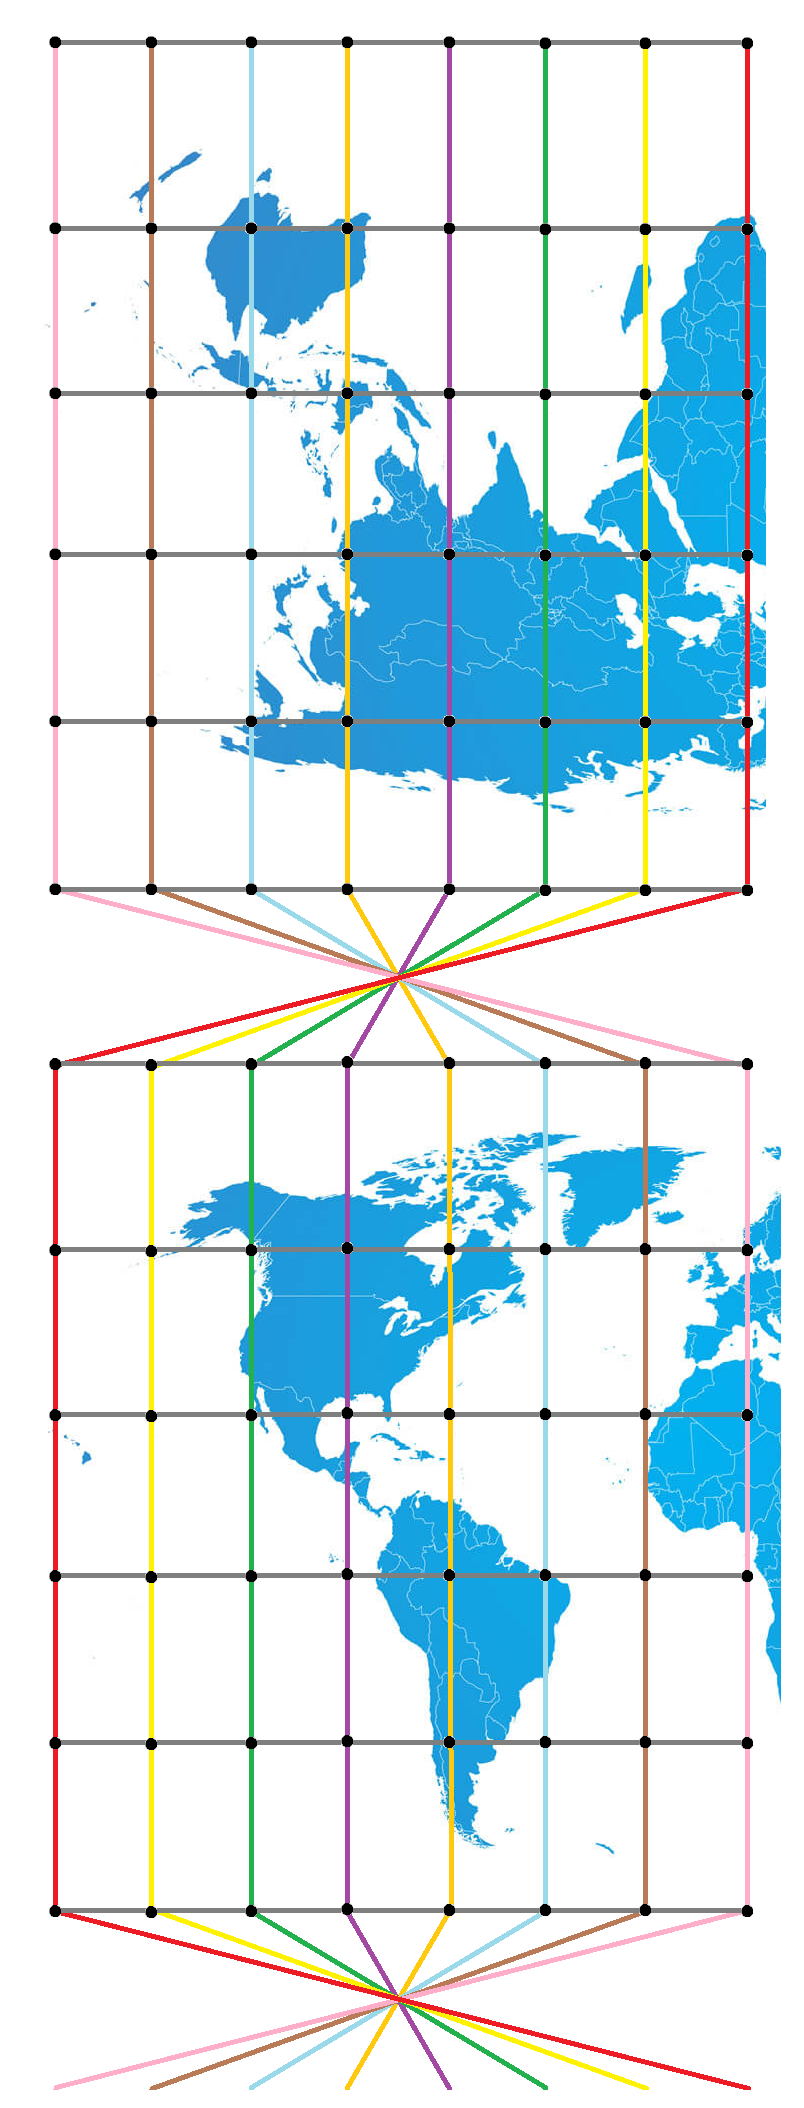
\includegraphics[scale=0.3]{network.png}
\caption[Shceme of the constellation]{Scheme of the constellation. Black dots are satellites. Color lines are communication links in the same orbital plane. Grey lines are links between orbital planes.}
\label{Scheme of the constellation}
\end{figure}